%%%% Paramétrage du TD %%%%
\def\xxactivite{TD 01 \ifprof -- Corrigé \else \fi }
\def\xxauteur{\textsl{Xavier Pessoles}}


\def\xxnumchapitre{Chapitre 1 \vspace{.2cm}}
\def\xxchapitre{\hspace{.12cm} Stabilité des systèmes}

\def\xxcompetences{%
\textsl{%
\textbf{Savoirs et compétences :}\\
\vspace{-.4cm}
\begin{itemize}[label=\ding{112},font=\color{ocre}] 
%\item \textit{Mod3.C2 : } pôles dominants et réduction de l’ordre du modèle : principe, justification
%\item \textit{Res2.C4 : } stabilité des SLCI : définition entrée bornée -- sortie bornée (EB -- SB)	
%\item \textit{Res2.C5 : } stabilité des SLCI : équation caractéristique	
\item \textit{Res2.C6 : } stabilité des SLCI : position des pôles dans le plan complexe
\item \textit{Res2.C7 : } stabilité des SLCI : marges de stabilité (de gain et de phase)
\end{itemize}
}}


\def\xxfigures{
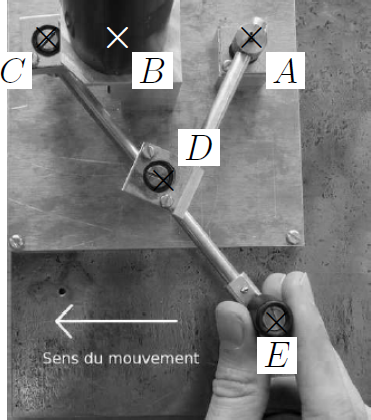
\includegraphics[width=.9\linewidth]{fig_00}
}%figues de la page de garde

\def\xxtitreexo{Robot pour la chirurgie endoscopique}
\def\xxsourceexo{\hspace{.2cm} \footnotesize{\textsl{Banque PT -- SIA -- 2005}}}


\iflivret
\pagestyle{empty}


%%%%%%%% PAGE DE GARDE COURS
\ifcours
% ==== BANDEAU DES TITRES ==== 
\begin{tikzpicture}[remember picture,overlay]
\node at (current page.north west)
{\begin{tikzpicture}[remember picture,overlay]
\node[anchor=north west,inner sep=0pt] at (0,0) {\includegraphics[width=\paperwidth]{\thechapterimage}};
\draw[anchor=west] (-2cm,-8cm) node [line width=2pt,rounded corners=15pt,draw=ocre,fill=white,fill opacity=0.6,inner sep=40pt]{\strut\makebox[22cm]{}};
\draw[anchor=west] (1cm,-8cm) node {\huge\sffamily\bfseries\color{black} %
\begin{minipage}{1cm}
\rotatebox{90}{\LARGE\sffamily\textsc{\color{ocre}\textbf{\xxnumpartie}}}
\end{minipage} \hfill
\begin{minipage}[c]{14cm}
\begin{titrepartie}
\begin{flushright}
\renewcommand{\baselinestretch}{1.1} 
\Large\sffamily\textsc{\textbf{\xxpartie}}
\renewcommand{\baselinestretch}{1} 
\end{flushright}
\end{titrepartie}
\end{minipage} \hfill
\begin{minipage}[c]{3.5cm}
{\large\sffamily\textsc{\textbf{\color{ocre} \discipline}}}
\end{minipage} 
 };
\end{tikzpicture}};
\end{tikzpicture}
% ==== FIN BANDEAU DES TITRES ==== 


% ==== ONGLET 
\begin{tikzpicture}[overlay]
\node[shape=rectangle, 
      rounded corners = .25 cm,
	  draw= ocre,
	  line width=2pt, 
	  fill = ocre!10,
	  minimum width  = 2.5cm,
	  minimum height = 3cm,] at (18.3cm,0) {};
\node at (17.7cm,0) {\rotatebox{90}{\textbf{\Large\color{ocre}{\classe}}}};
%{};
\end{tikzpicture}
% ==== FIN ONGLET 


\vspace{3.5cm}

\begin{tikzpicture}[remember picture,overlay]
\draw[anchor=west] (-2cm,-6cm) node {\huge\sffamily\bfseries\color{black} %
\begin{minipage}{2cm}
\begin{center}
\LARGE\sffamily\textsc{\color{ocre}\textbf{\xxactivite}}
\end{center}
\end{minipage} \hfill
\begin{minipage}[c]{15cm}
\begin{titrechapitre}
\renewcommand{\baselinestretch}{1.1} 
\Large\sffamily\textsc{\textbf{\xxnumchapitre}}

\Large\sffamily\textsc{\textbf{\xxchapitre}}
\vspace{.5cm}

\renewcommand{\baselinestretch}{1} 
\normalsize\normalfont
\xxcompetences
\end{titrechapitre}
\end{minipage}  };
\end{tikzpicture}
\vfill

\begin{flushright}
\begin{minipage}[c]{.3\linewidth}
\begin{center}
\xxfigures
\end{center}
\end{minipage}\hfill
\begin{minipage}[c]{.6\linewidth}
\startcontents
%\printcontents{}{1}{}
\printcontents{}{1}{}
\end{minipage}
\end{flushright}

\begin{tikzpicture}[remember picture,overlay]
\draw[anchor=west] (4.5cm,-.7cm) node {
\begin{minipage}[c]{.2\linewidth}
\begin{flushright}

\includegraphics[width=2cm]{logoCC}
\end{flushright}
\end{minipage}
\begin{minipage}[c]{.2\linewidth}
\textsl{\xxauteur} \\
\textsl{\classe}
\end{minipage}
 };
\end{tikzpicture}

\newpage
\pagestyle{fancy}

%\newpage
%\pagestyle{fancy}

\else
\fi
%% FIN PAGE DE GARDE DES COURS

%%%%%%%% PAGE DE GARDE TD
\iftd

% BANDEAU EXO
\iflivret % SI LIVRET
\begin{tikzpicture}[remember picture,overlay]
\draw[anchor=west] (-2cm,-3.3cm) node {\huge\sffamily\bfseries\color{black} %
\begin{minipage}{5cm}
\begin{center}
\LARGE\sffamily\color{ocre}\textbf{\textsc{\xxactivite}}

\begin{center}
\xxfigures
\end{center}

\end{center}
\end{minipage} \hfill
\begin{minipage}[c]{12cm}
\begin{titrechapitre}
\renewcommand{\baselinestretch}{1.1} 
\large\sffamily\textbf{\textsc{\xxtitreexo}}

\small\sffamily{\textbf{\textit{\color{black!70}\xxsourceexo}}}
\vspace{.5cm}

\renewcommand{\baselinestretch}{1} 
\normalsize\normalfont
\xxcompetences
\end{titrechapitre}
\end{minipage}};
\end{tikzpicture}
\else % ELSE NOT LIVRET
\begin{tikzpicture}[remember picture,overlay]
\draw[anchor=west] (-2cm,-4.5cm) node {\huge\sffamily\bfseries\color{black} %
\begin{minipage}{5cm}
\begin{center}
\LARGE\sffamily\color{ocre}\textbf{\textsc{\xxactivite}}

\begin{center}
\xxfigures
\end{center}

\end{center}
\end{minipage} \hfill
\begin{minipage}[c]{12cm}
\begin{titrechapitre}
\renewcommand{\baselinestretch}{1.1} 
\large\sffamily\textbf{\textsc{\xxtitreexo}}

\small\sffamily{\textbf{\textit{\color{black!70}\xxsourceexo}}}
\vspace{.5cm}

\renewcommand{\baselinestretch}{1} 
\normalsize\normalfont
\xxcompetences
\end{titrechapitre}
\end{minipage}};
\end{tikzpicture}

\fi

\else   % FIN IF TD
\fi


%%%%%%%% PAGE DE GARDE FICHE
\iffiche
\begin{tikzpicture}[remember picture,overlay]
\node at (current page.north west)
{\begin{tikzpicture}[remember picture,overlay]
\draw[anchor=west] (-2cm,-2.25cm) node [line width=2pt,rounded corners=15pt,draw=ocre,fill=white,fill opacity=0.6,inner sep=40pt]{\strut\makebox[22cm]{}};
\draw[anchor=west] (1cm,-2.25cm) node {\huge\sffamily\bfseries\color{black} %
\begin{minipage}{1cm}
\rotatebox{90}{\LARGE\sffamily\textsc{\color{ocre}\textbf{\xxnumpartie}}}
\end{minipage} \hfill
\begin{minipage}[c]{14cm}
\begin{titrepartie}
\begin{flushright}
\renewcommand{\baselinestretch}{1.1} 
\large\sffamily\textsc{\textbf{\xxpartie} \\} 

\vspace{.2cm}

\normalsize\sffamily\textsc{\textbf{\xxnumchapitre -- \xxchapitre}}
\renewcommand{\baselinestretch}{1} 
\end{flushright}
\end{titrepartie}
\end{minipage} \hfill
\begin{minipage}[c]{3.5cm}
{\large\sffamily\textsc{\textbf{\color{ocre} \discipline}}}
\end{minipage} 
 };
\end{tikzpicture}};
\end{tikzpicture}

\iflivret % SI LIVRET
\begin{tikzpicture}[overlay]
\node[shape=rectangle, 
      rounded corners = .25 cm,
	  draw= ocre,
	  line width=2pt, 
	  fill = ocre!10,
	  minimum width  = 2.5cm,
	  minimum height = 2.5cm,] at (18.5cm,.5cm) {};
\node at (17.9cm,.5cm) {\rotatebox{90}{\textsf{\textbf{\large\color{ocre}{\classe}}}}};
%{};
\end{tikzpicture}
\else  % SI PAS LIVRET
\iftd %% SI TD et PAS LIVRET
\begin{tikzpicture}[overlay]
\node[shape=rectangle, 
      rounded corners = .25 cm,
	  draw= ocre,
	  line width=2pt, 
	  fill = ocre!10,
	  minimum width  = 2.5cm,
	  minimum height = 2.5cm,] at (18.6cm,0.9cm) {};
\node at (18cm,0.9cm) {\rotatebox{90}{\textsf{\textbf{\large\color{ocre}{\classe}}}}};
%{};
\end{tikzpicture}

\else % FIN DU SI TD PAS LIVRET 
\begin{tikzpicture}[overlay]
\node[shape=rectangle, 
      rounded corners = .25 cm,
	  draw= ocre,
	  line width=2pt, 
	  fill = ocre!10,
	  minimum width  = 2.5cm,
%	  minimum height = 2.5cm,] at (18.5cm,1.1cm) {};
	  minimum height = 2.5cm,] at (18.6cm,0.5cm) {};
\node at (18cm,0.5cm) {\rotatebox{90}{\textsf{\textbf{\large\color{ocre}{\classe}}}}};
%{};
\end{tikzpicture}
\fi
\fi
\else
\fi



\else
\pagestyle{empty}


%%%%%%%% PAGE DE GARDE COURS
\ifcours
% ==== BANDEAU DES TITRES ==== 
\begin{tikzpicture}[remember picture,overlay]
\node at (current page.north west)
{\begin{tikzpicture}[remember picture,overlay]
\node[anchor=north west,inner sep=0pt] at (0,0) {\includegraphics[width=\paperwidth]{\thechapterimage}};
\draw[anchor=west] (-2cm,-8cm) node [line width=2pt,rounded corners=15pt,draw=ocre,fill=white,fill opacity=0.6,inner sep=40pt]{\strut\makebox[22cm]{}};
\draw[anchor=west] (1cm,-8cm) node {\huge\sffamily\bfseries\color{black} %
\begin{minipage}{1cm}
\rotatebox{90}{\LARGE\sffamily\textsc{\color{ocre}\textbf{\xxnumpartie}}}
\end{minipage} \hfill
\begin{minipage}[c]{14cm}
\begin{titrepartie}
\begin{flushright}
\renewcommand{\baselinestretch}{1.1} 
\Large\sffamily\textsc{\textbf{\xxpartie}}
\renewcommand{\baselinestretch}{1} 
\end{flushright}
\end{titrepartie}
\end{minipage} \hfill
\begin{minipage}[c]{3.5cm}
{\large\sffamily\textsc{\textbf{\color{ocre} \discipline}}}
\end{minipage} 
 };
\end{tikzpicture}};
\end{tikzpicture}
% ==== FIN BANDEAU DES TITRES ==== 


% ==== ONGLET 
\begin{tikzpicture}[overlay]
\node[shape=rectangle, 
      rounded corners = .25 cm,
	  draw= ocre,
	  line width=2pt, 
	  fill = ocre!10,
	  minimum width  = 2.5cm,
	  minimum height = 3cm,] at (18.3cm,0) {};
\node at (17.7cm,0) {\rotatebox{90}{\textbf{\Large\color{ocre}{\classe}}}};
%{};
\end{tikzpicture}
% ==== FIN ONGLET 


\vspace{3.5cm}

\begin{tikzpicture}[remember picture,overlay]
\draw[anchor=west] (-2cm,-6cm) node {\huge\sffamily\bfseries\color{black} %
\begin{minipage}{2cm}
\begin{center}
\LARGE\sffamily\textsc{\color{ocre}\textbf{\xxactivite}}
\end{center}
\end{minipage} \hfill
\begin{minipage}[c]{15cm}
\begin{titrechapitre}
\renewcommand{\baselinestretch}{1.1} 
\Large\sffamily\textsc{\textbf{\xxnumchapitre}}

\Large\sffamily\textsc{\textbf{\xxchapitre}}
\vspace{.5cm}

\renewcommand{\baselinestretch}{1} 
\normalsize\normalfont
\xxcompetences
\end{titrechapitre}
\end{minipage}  };
\end{tikzpicture}
\vfill

\begin{flushright}
\begin{minipage}[c]{.3\linewidth}
\begin{center}
\xxfigures
\end{center}
\end{minipage}\hfill
\begin{minipage}[c]{.6\linewidth}
\startcontents
%\printcontents{}{1}{}
\printcontents{}{1}{}
\end{minipage}
\end{flushright}

\begin{tikzpicture}[remember picture,overlay]
\draw[anchor=west] (4.5cm,-.7cm) node {
\begin{minipage}[c]{.2\linewidth}
\begin{flushright}

\includegraphics[width=2cm]{logoCC}
\end{flushright}
\end{minipage}
\begin{minipage}[c]{.2\linewidth}
\textsl{\xxauteur} \\
\textsl{\classe}
\end{minipage}
 };
\end{tikzpicture}

\newpage
\pagestyle{fancy}

%\newpage
%\pagestyle{fancy}

\else
\fi
%% FIN PAGE DE GARDE DES COURS

%%%%%%%% PAGE DE GARDE TD
\iftd

% BANDEAU EXO
\iflivret % SI LIVRET
\begin{tikzpicture}[remember picture,overlay]
\draw[anchor=west] (-2cm,-3.3cm) node {\huge\sffamily\bfseries\color{black} %
\begin{minipage}{5cm}
\begin{center}
\LARGE\sffamily\color{ocre}\textbf{\textsc{\xxactivite}}

\begin{center}
\xxfigures
\end{center}

\end{center}
\end{minipage} \hfill
\begin{minipage}[c]{12cm}
\begin{titrechapitre}
\renewcommand{\baselinestretch}{1.1} 
\large\sffamily\textbf{\textsc{\xxtitreexo}}

\small\sffamily{\textbf{\textit{\color{black!70}\xxsourceexo}}}
\vspace{.5cm}

\renewcommand{\baselinestretch}{1} 
\normalsize\normalfont
\xxcompetences
\end{titrechapitre}
\end{minipage}};
\end{tikzpicture}
\else % ELSE NOT LIVRET
\begin{tikzpicture}[remember picture,overlay]
\draw[anchor=west] (-2cm,-4.5cm) node {\huge\sffamily\bfseries\color{black} %
\begin{minipage}{5cm}
\begin{center}
\LARGE\sffamily\color{ocre}\textbf{\textsc{\xxactivite}}

\begin{center}
\xxfigures
\end{center}

\end{center}
\end{minipage} \hfill
\begin{minipage}[c]{12cm}
\begin{titrechapitre}
\renewcommand{\baselinestretch}{1.1} 
\large\sffamily\textbf{\textsc{\xxtitreexo}}

\small\sffamily{\textbf{\textit{\color{black!70}\xxsourceexo}}}
\vspace{.5cm}

\renewcommand{\baselinestretch}{1} 
\normalsize\normalfont
\xxcompetences
\end{titrechapitre}
\end{minipage}};
\end{tikzpicture}

\fi

\else   % FIN IF TD
\fi


%%%%%%%% PAGE DE GARDE FICHE
\iffiche
\begin{tikzpicture}[remember picture,overlay]
\node at (current page.north west)
{\begin{tikzpicture}[remember picture,overlay]
\draw[anchor=west] (-2cm,-2.25cm) node [line width=2pt,rounded corners=15pt,draw=ocre,fill=white,fill opacity=0.6,inner sep=40pt]{\strut\makebox[22cm]{}};
\draw[anchor=west] (1cm,-2.25cm) node {\huge\sffamily\bfseries\color{black} %
\begin{minipage}{1cm}
\rotatebox{90}{\LARGE\sffamily\textsc{\color{ocre}\textbf{\xxnumpartie}}}
\end{minipage} \hfill
\begin{minipage}[c]{14cm}
\begin{titrepartie}
\begin{flushright}
\renewcommand{\baselinestretch}{1.1} 
\large\sffamily\textsc{\textbf{\xxpartie} \\} 

\vspace{.2cm}

\normalsize\sffamily\textsc{\textbf{\xxnumchapitre -- \xxchapitre}}
\renewcommand{\baselinestretch}{1} 
\end{flushright}
\end{titrepartie}
\end{minipage} \hfill
\begin{minipage}[c]{3.5cm}
{\large\sffamily\textsc{\textbf{\color{ocre} \discipline}}}
\end{minipage} 
 };
\end{tikzpicture}};
\end{tikzpicture}

\iflivret % SI LIVRET
\begin{tikzpicture}[overlay]
\node[shape=rectangle, 
      rounded corners = .25 cm,
	  draw= ocre,
	  line width=2pt, 
	  fill = ocre!10,
	  minimum width  = 2.5cm,
	  minimum height = 2.5cm,] at (18.5cm,.5cm) {};
\node at (17.9cm,.5cm) {\rotatebox{90}{\textsf{\textbf{\large\color{ocre}{\classe}}}}};
%{};
\end{tikzpicture}
\else  % SI PAS LIVRET
\iftd %% SI TD et PAS LIVRET
\begin{tikzpicture}[overlay]
\node[shape=rectangle, 
      rounded corners = .25 cm,
	  draw= ocre,
	  line width=2pt, 
	  fill = ocre!10,
	  minimum width  = 2.5cm,
	  minimum height = 2.5cm,] at (18.6cm,0.9cm) {};
\node at (18cm,0.9cm) {\rotatebox{90}{\textsf{\textbf{\large\color{ocre}{\classe}}}}};
%{};
\end{tikzpicture}

\else % FIN DU SI TD PAS LIVRET 
\begin{tikzpicture}[overlay]
\node[shape=rectangle, 
      rounded corners = .25 cm,
	  draw= ocre,
	  line width=2pt, 
	  fill = ocre!10,
	  minimum width  = 2.5cm,
%	  minimum height = 2.5cm,] at (18.5cm,1.1cm) {};
	  minimum height = 2.5cm,] at (18.6cm,0.5cm) {};
\node at (18cm,0.5cm) {\rotatebox{90}{\textsf{\textbf{\large\color{ocre}{\classe}}}}};
%{};
\end{tikzpicture}
\fi
\fi
\else
\fi



\fi
\setlength{\columnseprule}{.1pt}

\pagestyle{fancy}
\thispagestyle{plain}


\vspace{4.5cm}

\def\columnseprulecolor{\color{ocre}}
\setlength{\columnseprule}{0.4pt} 

%%%%%%%%%%%%%%%%%%%%%%%



\begin{multicols}{2}
\setcounter{exo}{0}
\section*{Présentation}
On s’intéresse au robot de chirurgie endoscopique <<~Endoxirob~>>. Il est nécessaire de permettre à l’instrument chirurgical de se mouvoir avec des performances dynamiques comparables ou meilleures que celles réalisées par un chirurgien humain. 
L’étude est effectuée uniquement pour l’axe « d’élévation » selon $\vect{z_1}$. 


\begin{center}
\begin{tabular}{|c|p{4.4cm}|p{1.7cm}|}
\hline 
Req. & Exigence & Niveaux \\ \hline
1 & Vitesse de translation nominale & $>\SI{0,1}{m.s^{-1}}$ \\ \hline
2 & Temps $t_1$ pour atteindre la vitesse nominale & $\SI{100}{ms}$ maximum \\ \hline
3 & Précision -- Écart statique & $<\SI{0,2}{mm}$ \\ \hline
4 & Précision --  Retard de traînage pour une rampe de$ \SI{0,1}{m.s^{-1}}$  & $<\SI{0,1}{s}$ \\ \hline
5 & Stabilité -- Dépassement & Aucun \\ \hline
6 & Stabilité -- Marge de phase & $45\degres$ \\ \hline
7 & Rapidité -- Bande passante à \SI{-3}{dB} pour la partie mécanique & $\SI{4}{Hz}$ \\
\hline
\end{tabular}
\end{center}
La figure suivante présente le schéma-blocs de l'axe d’élévation (selon $\vect{Z_1}$) du dispositif de commande de l’instrument chirurgical. 

\begin{center}
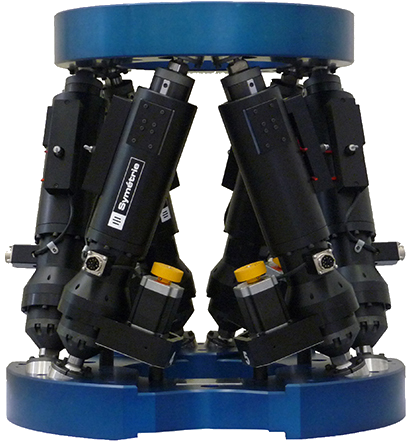
\includegraphics[width=\linewidth]{fig_01}
\end{center}

La console permet de capter le déplacement de la main, de le coder, de le corriger éventuellement afin d’élaborer la consigne de position angulaire du rotor moteur. 
La position angulaire est ensuite transformée en position linéaire de l’instrument par un mécanisme de transformation de mouvement à crémaillère.

La figure suivante présente de façon simplifiée, la chaîne cinématique de l’axe d’élévation :
\begin{itemize}
\item l’actionneur est un moto-réducteur (1) à courant continu Gammatic n° RH-8D-6006;
le premier étage de transmission du mouvement se fait par une courroie crantée (2) qui s’enroule sur des poulies de même diamètre pour entraîner l’arbre intermédiaire (3);
\item une roue dentée (3’) de diamètre primitif $\Phi_1 = \SI{38,4}{mm}$ solidaire de l’arbre intermédiaire (3) engrène avec une crémaillère (4) solidaire de la partie supérieure mobile du robot;
\item cette crémaillère est en liaison glissière d’axe $\vect{z_1}$ par rapport à la partie inférieure du robot considérée comme fixe dans cette partie du sujet, et notée « Bâti ».
\end{itemize}

Pour équilibrer le poids de la partie supérieure (coulisseau compris) de masse $M = \SI{5,5}{kg}$, les ingénieurs ont placé un contre-poids (7) de masse $2M = \SI{11}{kg}$ tiré par un câble qui s’enroule sur un tambour (3") de diamètre $\Phi_2 = \dfrac{\Phi}{2} = \SI{19,2}{mm}$ solidaire de  l’arbre intermédiaire (3).


\begin{center}
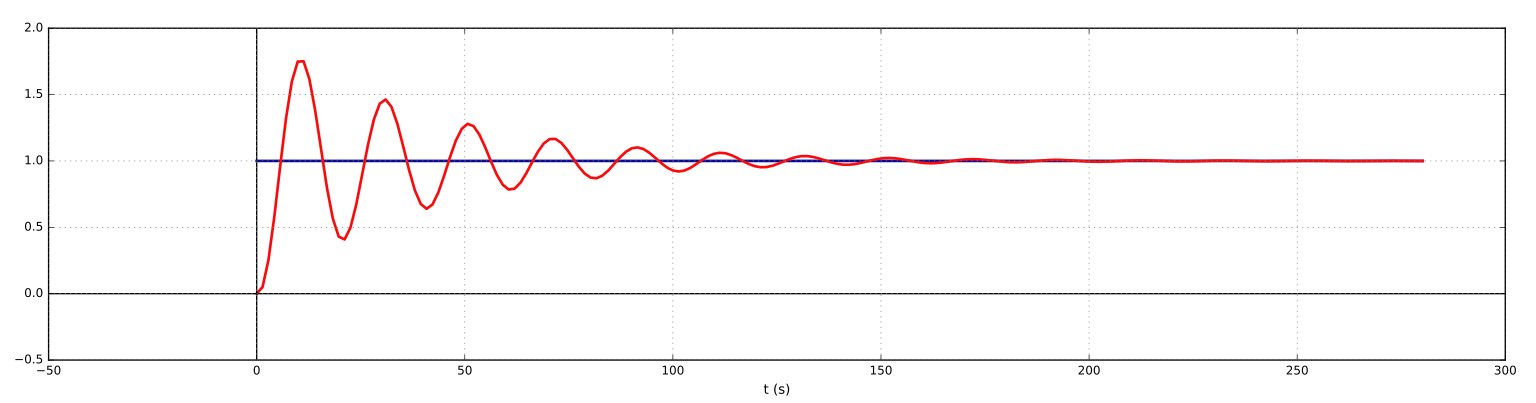
\includegraphics[width=\linewidth]{fig_02}
\end{center}



Le constructeur du moto-réducteur donne les caractéristiques mécaniques en sortie du réducteur  ce qui permet de considérer le moto-réducteur comme un « moteur qui tourne lentement avec un couple élevé » :
\begin{itemize}
\item puissance nominale en sortie du réducteur : $P_{\text{nom}} = \SI{8,6}{W}$;
\item couple nominal en sortie du réducteur : $C_{\text{nom }} = \SI{1,4}{Nm}$;  
\item couple de maintien en sortie du réducteur : $C_{\text{maint}} = \SI{1,5}{Nm}$;
\item couple maxi en sortie du réducteur : $C_{\text{max}}	= \SI{2,7}{Nm}$;
\item vitesse nominale en sortie du réducteur : $N_{\text{nom}} = \SI{60}{tr.min^{-1}}$;
\item vitesse maxi en sortie du réducteur : $N_{\text{max}} = \SI{100}{tr.min^{-1}}$;
\item moment d’inertie total ramené à l’arbre de sortie du réducteur : $J_1 = \SI{3,70e-3}{kg.m^2}$; 
\item capteur de position : codeur 360 incréments par tour monté sur le rotor du moteur;
\item rapport de réduction : 50 (n’interviendra que dans le calcul de la résolution du capteur).
\end{itemize}

\subsection*{Évaluation de la fonction de transfert du moto-réducteur}
Le constructeur donne les caractéristiques électro-mécaniques exprimées à la sortie du réducteur.
On rappelle les équations temporelles :
$u(t) = R i(t) + L \dfrac{\dd i(t)}{\dd t} + e(t)$, $e(t) = k_e  \omega_{\text{réd}}(t)$, 
$C_{\text{réd}} (t)= k_c  i(t)$, $C_{\text{réd}} (t) – C_r – f_v \omega_{\text{réd}}(t)= J_{\text{équ}} \dfrac{\dd \omega_{\text{réd}}(t)}{\dd t}$. 

Avec :
\begin{itemize}
\item $u(t)$ tension appliquée aux bornes de l’induit 
\item $i(t)$ intensité du courant traversant l’induit
\item $e(t)$ force électromotrice induite par la rotation du moteur, évaluée à la  sortie du réducteur;
\item $\omega_{\text{réd}}(t)$ vitesse de rotation à la sortie du réducteur;
\item $C_{\text{réd}} (t)$ couple moteur ramené à la sortie du réducteur;
\item $R = \SI{10}{W}$ : résistance de l’induit;
\item $L = \SI{2,2}{mH}$ inductance de l’induit;
\item $k_c = \SI{2,1}{N.m.A^{-1}}$ constante de couple évaluée à la sortie du réducteur;
\item $k_e = \SI{2,1}{V.s.rad^{-1}}$ constante de f.e.m évaluée à la sortie du réducteur;
\item $C_r = \SI{0,2}{N.m}$ couple résistant induit par les frottements secs, ramené à la sortie du réducteur 
\item $f_v = \SI{0,04}{Nm.s.rad^{-1}}$ coefficient de frottement visqueux équivalent à toutes les pièces en mouvement, ramené à la sortie du réducteur 
\item $J_{\text{équ}} = \SI{7e-3}{kg.m^2}$ moment d’inertie équivalent à toutes les pièces en mouvement, ramené à la sortie du réducteur. 
\end{itemize}

Les transformées de Laplace des fonctions $u(t)$, $i(t)$, $e(t)$, $\omega_{\text{réd}}(t)$,  $C_{\text{réd}}(t)$ sont respectivement $U(p)$, $I(p)$, $E(p)$, $\Omega_{\text{réd}}(p)$ et $C_{\text{réd}}(p)$. On considère toutes les conditions initiales nulles.

\subparagraph{}\textit{Transformer les équations temporelles ci-dessus. 
Remplir sous forme littérale les blocs du schéma suivant. Exprimer les grandeurs physiques entre chaque bloc. }
\ifprof
\begin{corrige}
\end{corrige}
\else
\fi

\begin{center}
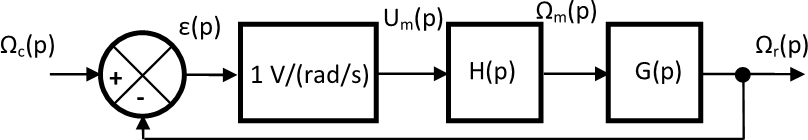
\includegraphics[width=\linewidth]{fig_03}
\end{center}


\subparagraph{}\textit{Exprimer littéralement sous forme canonique la fonction de transfert du moto-réducteur $M(p)=\dfrac{\Omega_{\text{réd}}(p)}{U(p)}$.}
\ifprof
\begin{corrige}
\end{corrige}
\else
\fi

Quel que soit le résultat obtenu à la question précédente, on utilisera l’expression de $M(p)$ suivante : $M_1(p)=\dfrac{0,436}{1+14,5\cdot 10^{-3}p+3,1\cdot 10^{-6}p^2}$. 

Sur le système de levage non asservi c’est à dire avec le capteur de position angulaire déconnecté, on a pratiqué, un essai en charge, en donnant au moteur un échelon de tension $u(t) = \SI{24}{V}$. 
Avec une génératrice tachymétrique dont le gain est de $\SI{0,166}{V.s.rad^{-1}}$ , on a tracé la courbe de tension image de $\omega_{\text{réd}}(t)$.  

\begin{center}
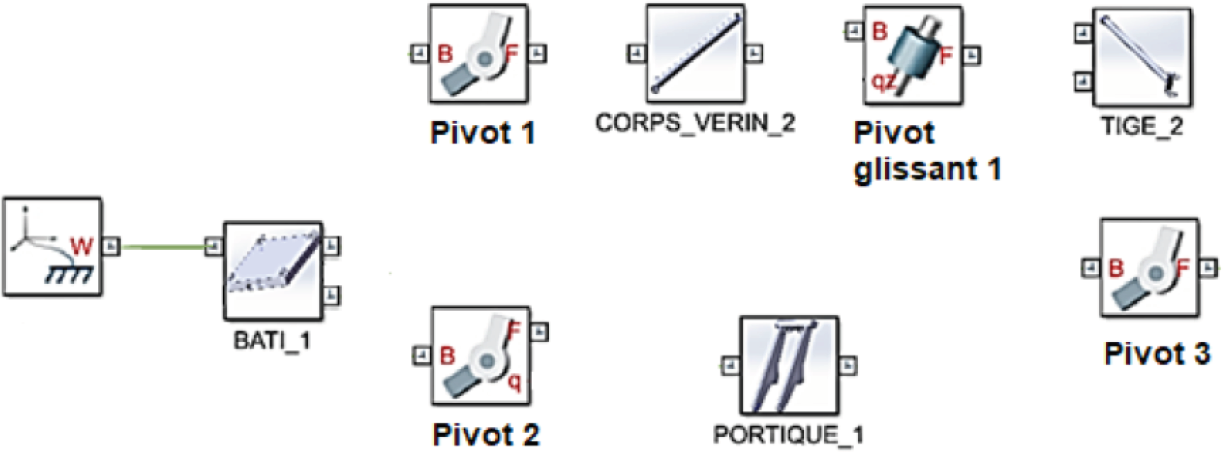
\includegraphics[width=\linewidth]{fig_04}
\end{center}


Remarque : la partie supérieure du robot est supposée rigide pendant cet essai.


\subparagraph{}\textit{Après avoir analysé cette courbe, expliquer pourquoi on peut négliger l’inductance $L$.}
\ifprof
\begin{corrige}
\end{corrige}
\else
\fi


\subparagraph{}\textit{Justifier analytiquement la réponse précédente à partir de l’expression de $M_1(p)$ lorsque l’on envisage une étude fréquentielle : on précisera la valeur du pôle dominant, l’autre (faisant intervenir la valeur de $L$) étant rejeté.}
*****
\ifprof
\begin{corrige}
\end{corrige}
\else
\fi

\textbf{Dans la suite du problème, on néglige l’inductance $L$ du moteur.}

\subparagraph{}\textit{Exprimer littéralement, sous forme canonique, la fonction de transfert du moto-réducteur  $M_2(p)=\dfrac{\Omega_{\text{réd}}(p)}{U(p)}=\dfrac{Gs}{1+Tp}$.  
Donner les valeurs numériques de $Gs$ et de $T$ à partir de l’expression de $M_1(p)$ et des réponses apportées précédemment.}
\ifprof
\begin{corrige}
\end{corrige}
\else
\fi


\subparagraph{}\textit{Déterminer les valeurs de $Gs$ et $T$, à partir de la courbe de tension image de $\omega_{\text{réd}}(t)$  (expliquer les démarches sous la figure et comparer avec les résultats obtenus précédemment). }
\ifprof
\begin{corrige}
\end{corrige}
\else
\fi

\subsection*{Respect du critère de marge de phase}
La boucle d’asservissement de la position angulaire de l’arbre de sortie du réducteur est définie par le schéma-blocs figure suivante. 
La consigne de position en incréments est élaborée par le  calculateur, à partir des informations envoyées par la console.

\begin{center}
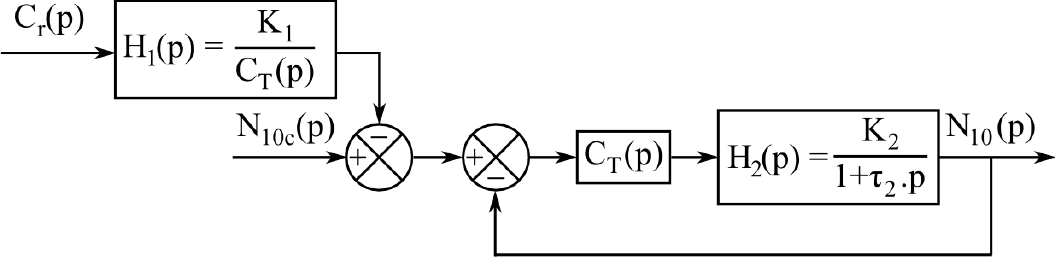
\includegraphics[width=\linewidth]{fig_05}
\end{center}


Le convertisseur-amplificateur $K$ de gain $k$ variable élabore la commande du moteur.
Le codeur incrémental $C$ placé sur le rotor du moteur a une résolution de 360 incréments par tour. Il est associé à un compteur -- décompteur qui élabore la mesure de position en incréments. 
Le système est discret (non continu) mais on l’assimile à un système continu car le comptage est très rapide. 
Le réducteur a un rapport de réduction de 50.
 
\subparagraph{}\textit{Donner la fonction de transfert du bloc $B(p)$ et la valeur du coefficient du bloc $C$ en incr./rad.  
Exprimer numériquement, en fonction de $k$, la fonction de transfert en boucle ouverte $H_O(p)$ .}
\ifprof
\begin{corrige}
\end{corrige}
\else
\fi


\subparagraph{}\textit{Tracer les diagrammes de Bode du système en boucle ouverte pour $k = 1$.
Le système est-il stable en boucle fermée pour cette valeur de $k$ ? Justifier.
} *****
\ifprof
\begin{corrige}
\end{corrige}
\else
\fi

********
On a tracé sur le document réponses figure R28 le diagramme de Black du système en boucle ouverte pour k = 1 lorsque la valeur de $L$ n’est pas négligée.
 
Question 28. : 
Quelle est l’influence de la prise en compte de $L$ sur la stabilité en boucle fermée ? (répondre sur le document réponses sous la figure R28). L’hypothèse consistant à négliger $L$ est-elle vérifiée ?
Déterminer, et expliquer à partir de constructions faites sur le diagramme de Black document réponses figure R28, la valeur $k_{45}$ de $k$ qui permet d’obtenir la marge de phase de 45\degres  spécifiée dans le cahier des charges.
*********


\subparagraph{}\textit{Calculer, pour la valeur $k_{45}$ de $k$ établie précédemment, l’écart statique $\varepsilon_{\text{cons} \infty}$ en incréments lorsque la consigne est un échelon de position : $\text{Cons}(t) = 1\cdot u(t)$.}
\ifprof
\begin{corrige}
\end{corrige}
\else
\fi


Étant donné que la perturbation $Cr$ intervient entre deux blocs de $M(p)$, on adopte le schéma de la 
figure suivante pour faciliter les calculs de la question suivante. 

\begin{center}
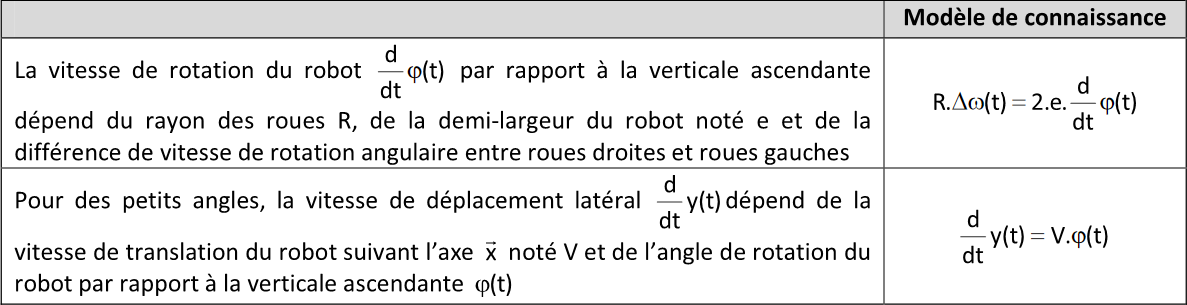
\includegraphics[width=\linewidth]{fig_06}
\end{center}


\subparagraph{}\textit{Calculer, pour la valeur $k_{45}$ de $k$ établie précédemment, l’écart statique $\varepsilon_{\text{pert} \infty}$ en incréments entre la consigne et la mesure lorsque la perturbation est l’échelon de couple résistant $C_r u(t)$ induit par les frottements secs. }
\ifprof
\begin{corrige}
\end{corrige}
\else
\fi


\subparagraph{}\textit{La chaîne cinématique de transmission est telle qu’il faut 150 incréments pour que la crémaillère se déplace de $\SI{1}{mm}$, quelle est l’incidence de cet écart sur la position de l’instrument ? }
\ifprof
\begin{corrige}
\end{corrige}
\else
\fi


\subparagraph{}\textit{Conclure par rapport aux exigences du cahier des charges.
Proposer une modification du bloc $K$ qui annulerait cet écart.}
\ifprof
\begin{corrige}
\end{corrige}
\else
\fi

\subsection*{Vérification des performances de la chaîne de positionnement de l'instrument}
\subsubsection*{Modélisation par schéma-blocs}

\begin{center}
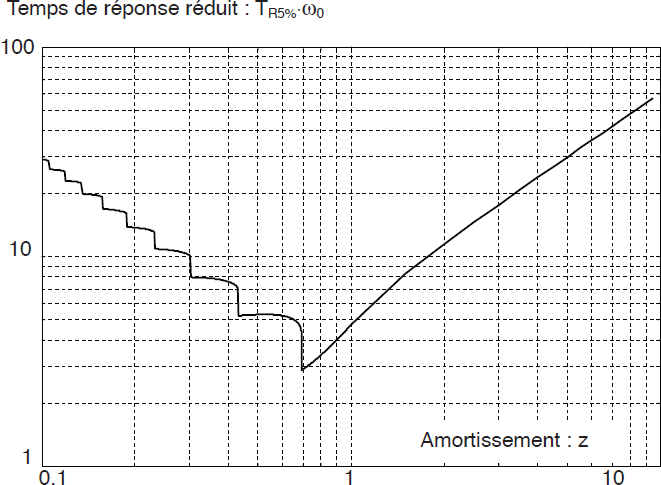
\includegraphics[width=\linewidth]{fig_07}
\end{center}


\subsubsection*{Analyse du déplacement en translation de la crémaillère}
Lorsque la boucle d’asservissement est bien réglée, la fonction de transfert est : $H_1(p)=\dfrac{\Theta(p)}{\text{Cons}(p)} = \dfrac{0,00035}{1+0,014p+0,00017 p^2}$. 
On rappelle que la courroie s’enroule sur des poulies de même diamètre et que la roue dentée qui engrène avec la crémaillère a un diamètre $\Phi_1 = \SI{38,4}{mm}$.


\subparagraph{}\textit{Exprimer le coefficient du bloc $H_2$; préciser l’unité.}
\ifprof
\begin{corrige}
\end{corrige}
\else
\fi

En régime statique, la position de la crémaillère est l’image de la position de la main, aux écarts près. 

\subparagraph{}\textit{Quelle relation doit vérifier le produit $P$ des gains des blocs $C_1$ , $H_1$ , $H_2$  ? Justifier.
Exprimer le coefficient $c_1$ en incréments par mètre du bloc $C_1$ .
}
\ifprof
\begin{corrige}
\end{corrige}
\else
\fi

Pour augmenter la précision de l’opération chirurgicale, on désire que la crémaillère se déplace 10 fois moins que la main. 




\subparagraph{}\textit{Exprimer le nouveau coefficient $c_2$ du bloc $C_1$ ainsi que le nouveau produit  $P_1$ . }
\ifprof
\begin{corrige}
\end{corrige}
\else
\fi

\subsubsection*{Analyse du déplacement de l’instrument chirurgical par rapport à la crémaillère}

La partie supérieure du robot est constituée par assemblage de tubes minces en fibres de carbone. 
On modélise cette partie par deux solides : $S_0$ représentant la crémaillère et les solides qui y sont liés ;  et $S_1$ représentant l’instrument chirurgical. 
Ces solides sont considérés en liaison glissière parfaite et reliés par un ressort de raideur $k_0$ et un amortisseur de coefficient $f_0$, montés en parallèle comme le montre le schéma.

\begin{center}
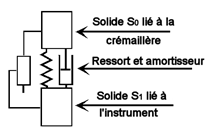
\includegraphics[width=.7\linewidth]{fig_09}
\end{center}

Pour identifier la fonction de transfert $H_3(p)=\dfrac{D_{\text{instrum}}(p)}{D_{\text{crem}}(p)}$ de cette partie, on a imposé à la crémaillère un échelon de déplacement $d_{\text{crém}}(t) = \SI{20e-3}{m}$ à partir de la position d’équilibre. On a tracé la courbe de déplacement $d_{\text{instrum}}(t)$ de l’instrument.

\begin{center}
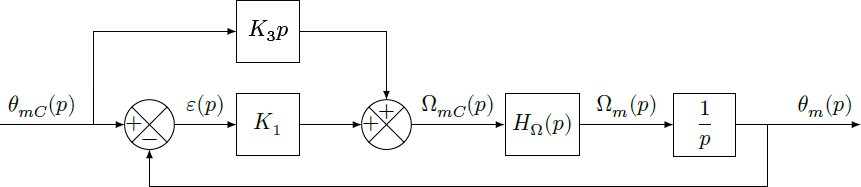
\includegraphics[width=\linewidth]{fig_08}
\end{center}

On donne sur la figure suivante les abaques des dépassements relatifs et des temps de réponse réduits d’un système du second ordre.

\begin{center}
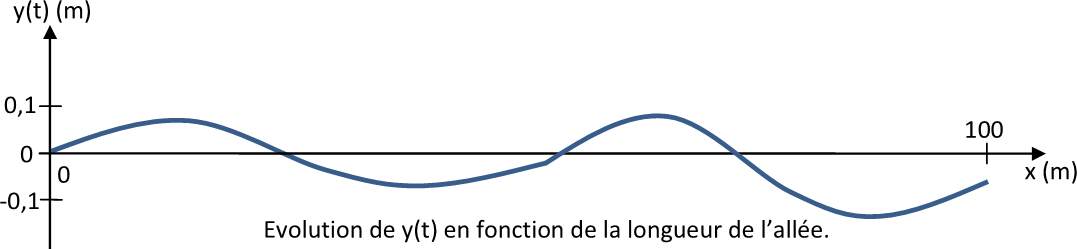
\includegraphics[width=\linewidth]{fig_10}
\end{center}


\subparagraph{}\textit{Établir, à partir de cette figure, l’expression de la fonction de transfert $H_3(p)$; déterminer les valeurs caractéristiques : gain statique, coefficient d’amortissement et pulsation propre.}
\ifprof
\begin{corrige}
\end{corrige}
\else
\fi


\subparagraph{}\textit{Le critère de la bande passante de \SI{4}{Hz} à  \SI{-3}{dB} est-il satisfait ? répondre et justifier sur le document réponse.}
\ifprof
\begin{corrige}
\end{corrige}
\else
\fi



Les questions suivantes vont permettre de déterminer l’expression analytique de $H_3(p)$, de façon à analyser l’influence du paramètre de raideur, pour respecter le critère de bande passante du cahier des charges.

Soit $m_1$ la masse du solide $S_1$. L’axe du mouvement est vertical ascendant et noté $\vect{z}$. L’origine $O$ du mouvement de $S_1$ correspond à la position pour laquelle le ressort est à sa longueur libre.
Soit $a_0$ l’allongement du ressort dans la position d’équilibre qui prend en compte l’action de la pesanteur. 
Nota : $a_0$ est négatif car on considère qu’il y a allongement du ressort.

L'équation du mouvement du ressort autour de la position d'équilibre est donné par : $m_1\dfrac{\dd^2 z(t)}{\dd t^2} + f_0 \dfrac{\dd z (t)}{\dd t}+k_0 z = 0$.

\subparagraph{}\textit{Après avoir mis l’équation différentielle du mouvement sous forme canonique : $\ddot{z}(t)+B\dot{z}(t)+z(t)=0$, exprimer le coefficient d’amortissement $\xi_3$ et la pulsation propre $\omega_{03}$ du mouvement en fonction de $k_0$, $f_0$, $m_1$ .}
\ifprof
\begin{corrige}
\end{corrige}
\else
\fi

On donne la valeur numérique de la masse de l’instrument chirurgical et de la plaque d’interface : $m_1 = \SI{1,6}{kg}$.


\subparagraph{}\textit{Pour la valeur de $\omega_{03}$ calculée précédemment, déterminer la valeur minimale de la raideur $k_0$ (en N/m) qui permettrait de respecter le critère de la bande passante à $\SI{-3}{dB}$ de \SI{4}{Hz}.
(On notera que $ \omega_{-\SI{3}{dB}}> \omega_{03}$).
}
\ifprof
\begin{corrige}
\end{corrige}
\else
\fi

\subsubsection{Analyse du déplacement de l’instrument par rapport au déplacement de la main}

On conserve la valeur $c_1$ du bloc $C_1$. La fonction de transfert du système est : $H(p)=\dfrac{D_{\text{instrum}}(p)}{D_{\text{main}}(p)}=\dfrac{1}{\left(1+0,014p+0,00017p^2 \right)\left( 1+0,015p+0,0014p^2\right)}$ .
Le chirurgien impose avec sa main une rampe de déplacement  de \SI{100}{mm.s^{-1}}. On a tracé sur la figure suivante les les courbes de déplacement de la main et de l’instrument.


\begin{center}
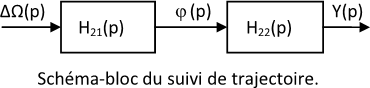
\includegraphics[width=\linewidth]{fig_11}
\end{center}


\subparagraph{}\textit{Mettre en évidence et donner les valeurs numériques :
de l’écart dynamique maximal; de l’écart de traînage (ou de vitesse) $\varepsilon_v$ en régime établi, du retard de traînage. Le cahier des charges est-il satisfait pour ce dernier critère ?
}
\ifprof
\begin{corrige}
\end{corrige}
\else
\fi


On donne, la courbe d’amplitude (gain) de $H(p)$ pour $p = j\omega$ dans le plan de Bode. 
La main du chirurgien est prise d’un tremblement sensiblement sinusoïdal dont la période est de \SI{0,25}{s} et l’amplitude \SI{1}{mm}. 


\begin{center}
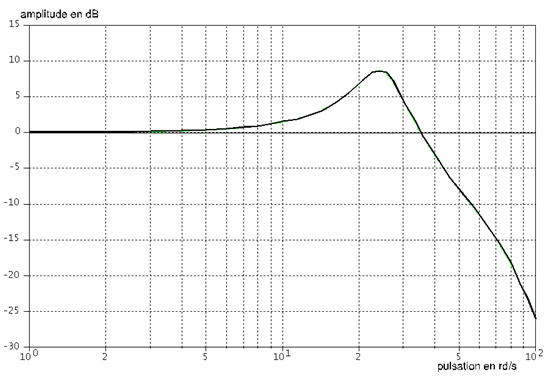
\includegraphics[width=\linewidth]{fig_12}
\end{center}

\subparagraph{}\textit{Déterminer à partir de cette courbe, l’amplitude du mouvement pris par l’instrument. Quelle est la conséquence de ce mouvement sur la plaie chirurgicale ?}
\ifprof
\begin{corrige}
\end{corrige}
\else
\fi

\subsubsection*{Amélioration des performances dynamiques}

On souhaite limiter l’amplitude du mouvement de l’outil lors du tremblement de la main en  filtrant le signal traité par le capteur-codeur $C_1$ de sorte que les tremblements n’apparaissent plus sur le soustracteur. On propose trois filtres du premier ordre, de gains statiques égaux à 1 et de constantes de temps :	 $T_1 = \SI{0,04}{s}$ ; $T_2 = \SI{0,1}{s}$; $T_3 = \SI{0,5}{s}$.



\subparagraph{}\textit{Tracer sur la figure précédente, les trois courbes asymptotiques d’amplitude de ces filtres avec des couleurs différentes. 
Sachant que les mouvements dont la période est inférieure à \SI{1}{s} ne doivent pas être atténués de plus de \SI{1}{dB}, choisir le numéro 1, 2 ou 3 du filtre qui atténue de 8 à \SI{10}{dB} le tremblement de la main de période \SI{0,25}{s}. 
Tracer sur cette figure, dans une autre couleur, l’allure de la courbe d’amplitude corrigée par ce filtre.
Le niveau de \SI{4}{Hz}, de la bande passante à $-\SI{3}{dB}$ du critère de rapidité est-il toujours respecté ? 
}
\ifprof
\begin{corrige}
\end{corrige}
\else
\fi
%
%\subparagraph{}\textit{}
%\ifprof
%\begin{corrige}
%\end{corrige}
%\else
%\fi
%
%\subparagraph{}\textit{}
%\ifprof
%\begin{corrige}
%\end{corrige}
%\else
%\fi
%
%\subparagraph{}\textit{}
%\ifprof
%\begin{corrige}
%\end{corrige}
%\else
%\fi

\end{multicols}
%\end{document}
%
%\subparagraph{}\textit{}
%
%
%\begin{center}
%\includegraphics[width=\linewidth]{}
%\end{center}
%
%\begin{center}
%\includegraphics[width=\linewidth]{}
%\textit{}
%\end{center}
%
